
% JuliaCon proceedings template
\documentclass{juliacon}
\setcounter{page}{1}

% my commands
\usepackage[absolute]{textpos}
\usepackage[nolist]{acronym}

\begin{acronym}[Bash]
	\acro{SDN}{Software-Defined Networking}
    \acro{BGP}{Border Gateway Protocol}
    \acro{MD}{multi-domain}
    \acro{NBI}{Northbound Interface}
    \acro{IBN}{Intent-Based Networking}
	\acro{DAG}{Directed Acyclic Graph}
	\acro{MSA}{Multi-Source Agreement}
	\acro{OXC}{Optical Cross-Connect}
    \acro{API}{Application Programming Interface}
\end{acronym}


\begin{document}


% **************GENERATED FILE, DO NOT EDIT**************

\title{MINDFul.jl: A Framework for Intent-driven Multi-Domain Network coordination}

\author[1]{Filippos Christou}
\affil[1]{Institute of Communication Networks and Computer Engineering (IKR), University of Stuttgart}

\keywords{Julia, Intent-based Networking, multi-domain, IP-optical}

\hypersetup{
pdftitle = {MINDFul.jl: A Framework for Intent-driven Multi-Domain Network coordination},
pdfsubject = {JuliaCon 2023 Proceedings},
pdfauthor = {Filippos Christou},
pdfkeywords = {Julia, Intent-based Networking, multi-domain, IP-optical},
}



\maketitle

\begin{textblock}{13.5}(3.4,1.6)
    {\color{blue}
    This work has been accepted in JuliaCon 2023 and will be submitted in the proceedings. The related contribution is https://pretalx.com/juliacon2023/talk/review/YR83GQLFDC37NXFF7GFRV7LKGXHCVRWT 
    }
\end{textblock}

\begin{abstract}
    Network coordination across multiple domains is a complex task requiring seamless communication between network entities.
    Network operators target to minimize costs while ensuring the requirements of the user requests.
    Such efforts are highly challenging in decentralized environments with diverse network operators, where only partial knowledge of the complete network is available.
    Intent-driven multi-domain coordination offers various benefits, some inherent to \ac{IBN} and others stemming from the standardization of the \ac{NBI}.
    As standardization is still missing, there has not been a substantial initiative to develop tools that leverage this paradigm.
    \verb|MINDFul.jl| is a Julia library that fills this gap and provides the means to accelerate research in this area, both at the architectural and the algorithmic level.
    It provides a stateful, modular representation of common metro/core IP-optical network equipment as well as the common intent operations.
    Finally, it facilitates event-based simulations with a hackable interface and offers visualization support.
\end{abstract}

\acresetall


\section{Background}
    As \ac{SDN} \cite{2015SDN} becomes more popular and many networks shift to centralized control due to easier management and higher efficiency, \ac{MD} networking often must remain decentralized due to its very nature.
    This will cause most of the networks to operate using a centralized \ac{SDN} controller internally but still need to coordinate in a decentralized fashion with the neighboring domains, as shown in Figure~\ref{fig:DeCentralized}.

    An intent-driven approach \cite{2023ietf, 2022ChristouCNSM} has been proposed, which can substitute traditional \ac{MD} decentralized protocols like the \ac{BGP} since they offer higher flexibility of interactions and support for much wider network capabilities.
    \ac{IBN} provides a layer of abstraction where high-level objectives (i.e., intents) can be defined and automatically handled by the system.
    Several design and algorithmic decisions need to be made to develop an \ac{IBN} framework, like the definition of an intent state machine and the algorithms that enable the state transitions.
    Commonly, an intent has at least the following four states, although naming conventions might differ:
    \begin{itemize}
        \item \emph{uncompiled} for unprocessed intents inside the system
        \item \emph{compiled} for processed intents with a well-defined implementation
        \item \emph{installed} for active intents whose implementation has been realized in the appropriate network devices
        \item \emph{failed} for active intents that malfunction after some failure during operation.
    \end{itemize}
    Several algorithms need to be provisioned, among which the most important deal with:
    \begin{itemize}
        \item \emph{intent compilation} for deriving an intent implementation and transitioning an intent to the compiled state
        \item \emph{intent monitoring} for reassuring that the installed intents satisfy all the requirements and trigger some fallbacks in case of failure
        \item \emph{intent conflict resolution} for handling situations when several intents require the same resources.
    \end{itemize}


    \begin{figure}[t]
    \centerline{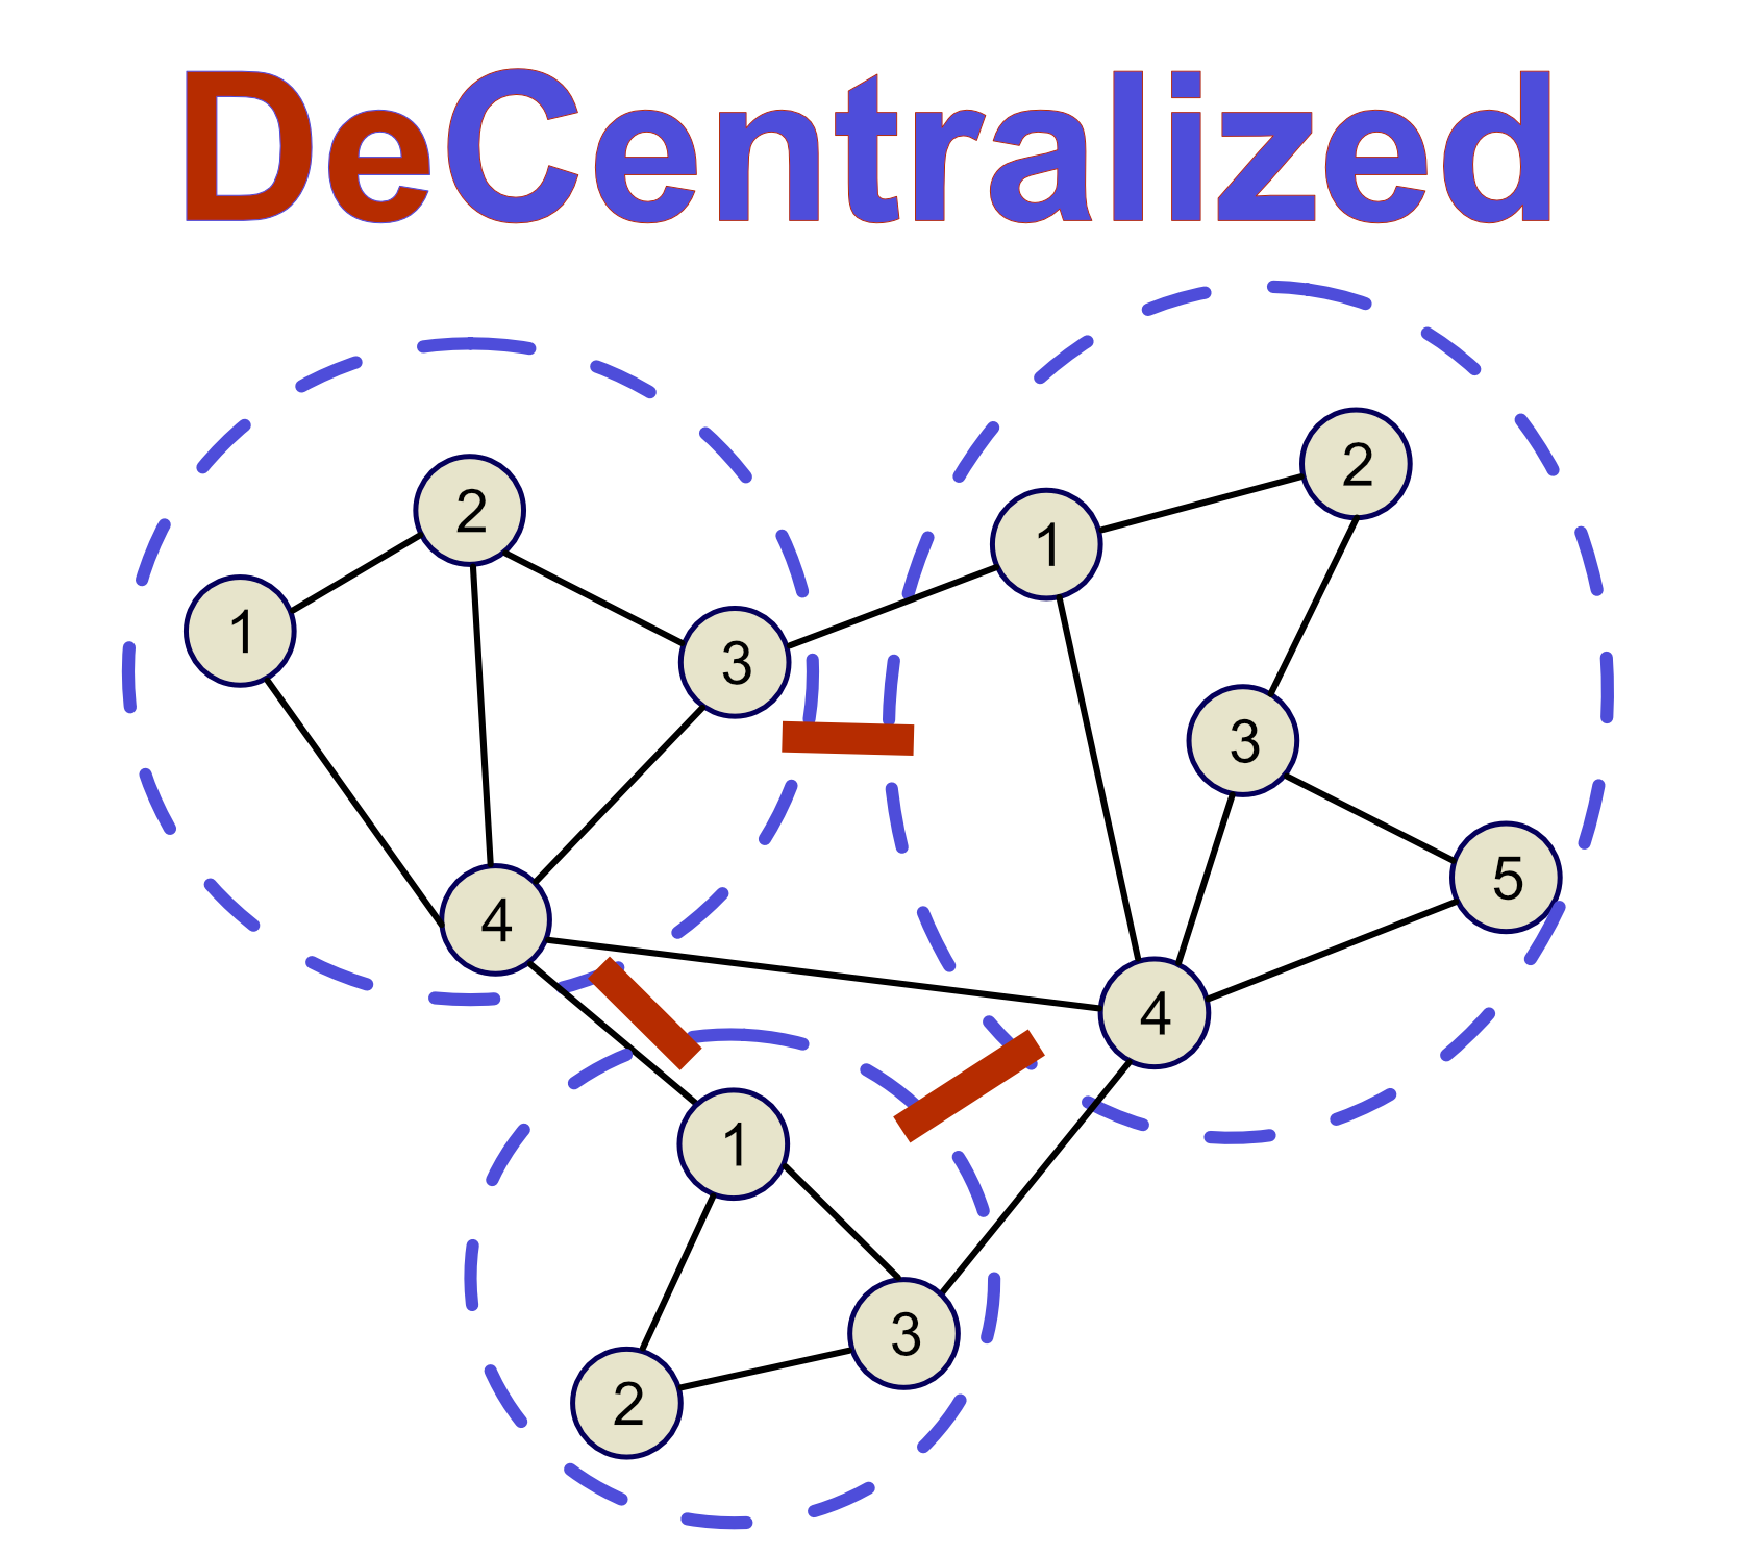
\includegraphics[width=5cm]{Motive.pdf}}
    \caption{Domains coordinate with each other in a decentralized fashion, while each domain has centralized control internally.}
        \label{fig:DeCentralized}
    \end{figure}

    \begin{figure}[b]
    \centerline{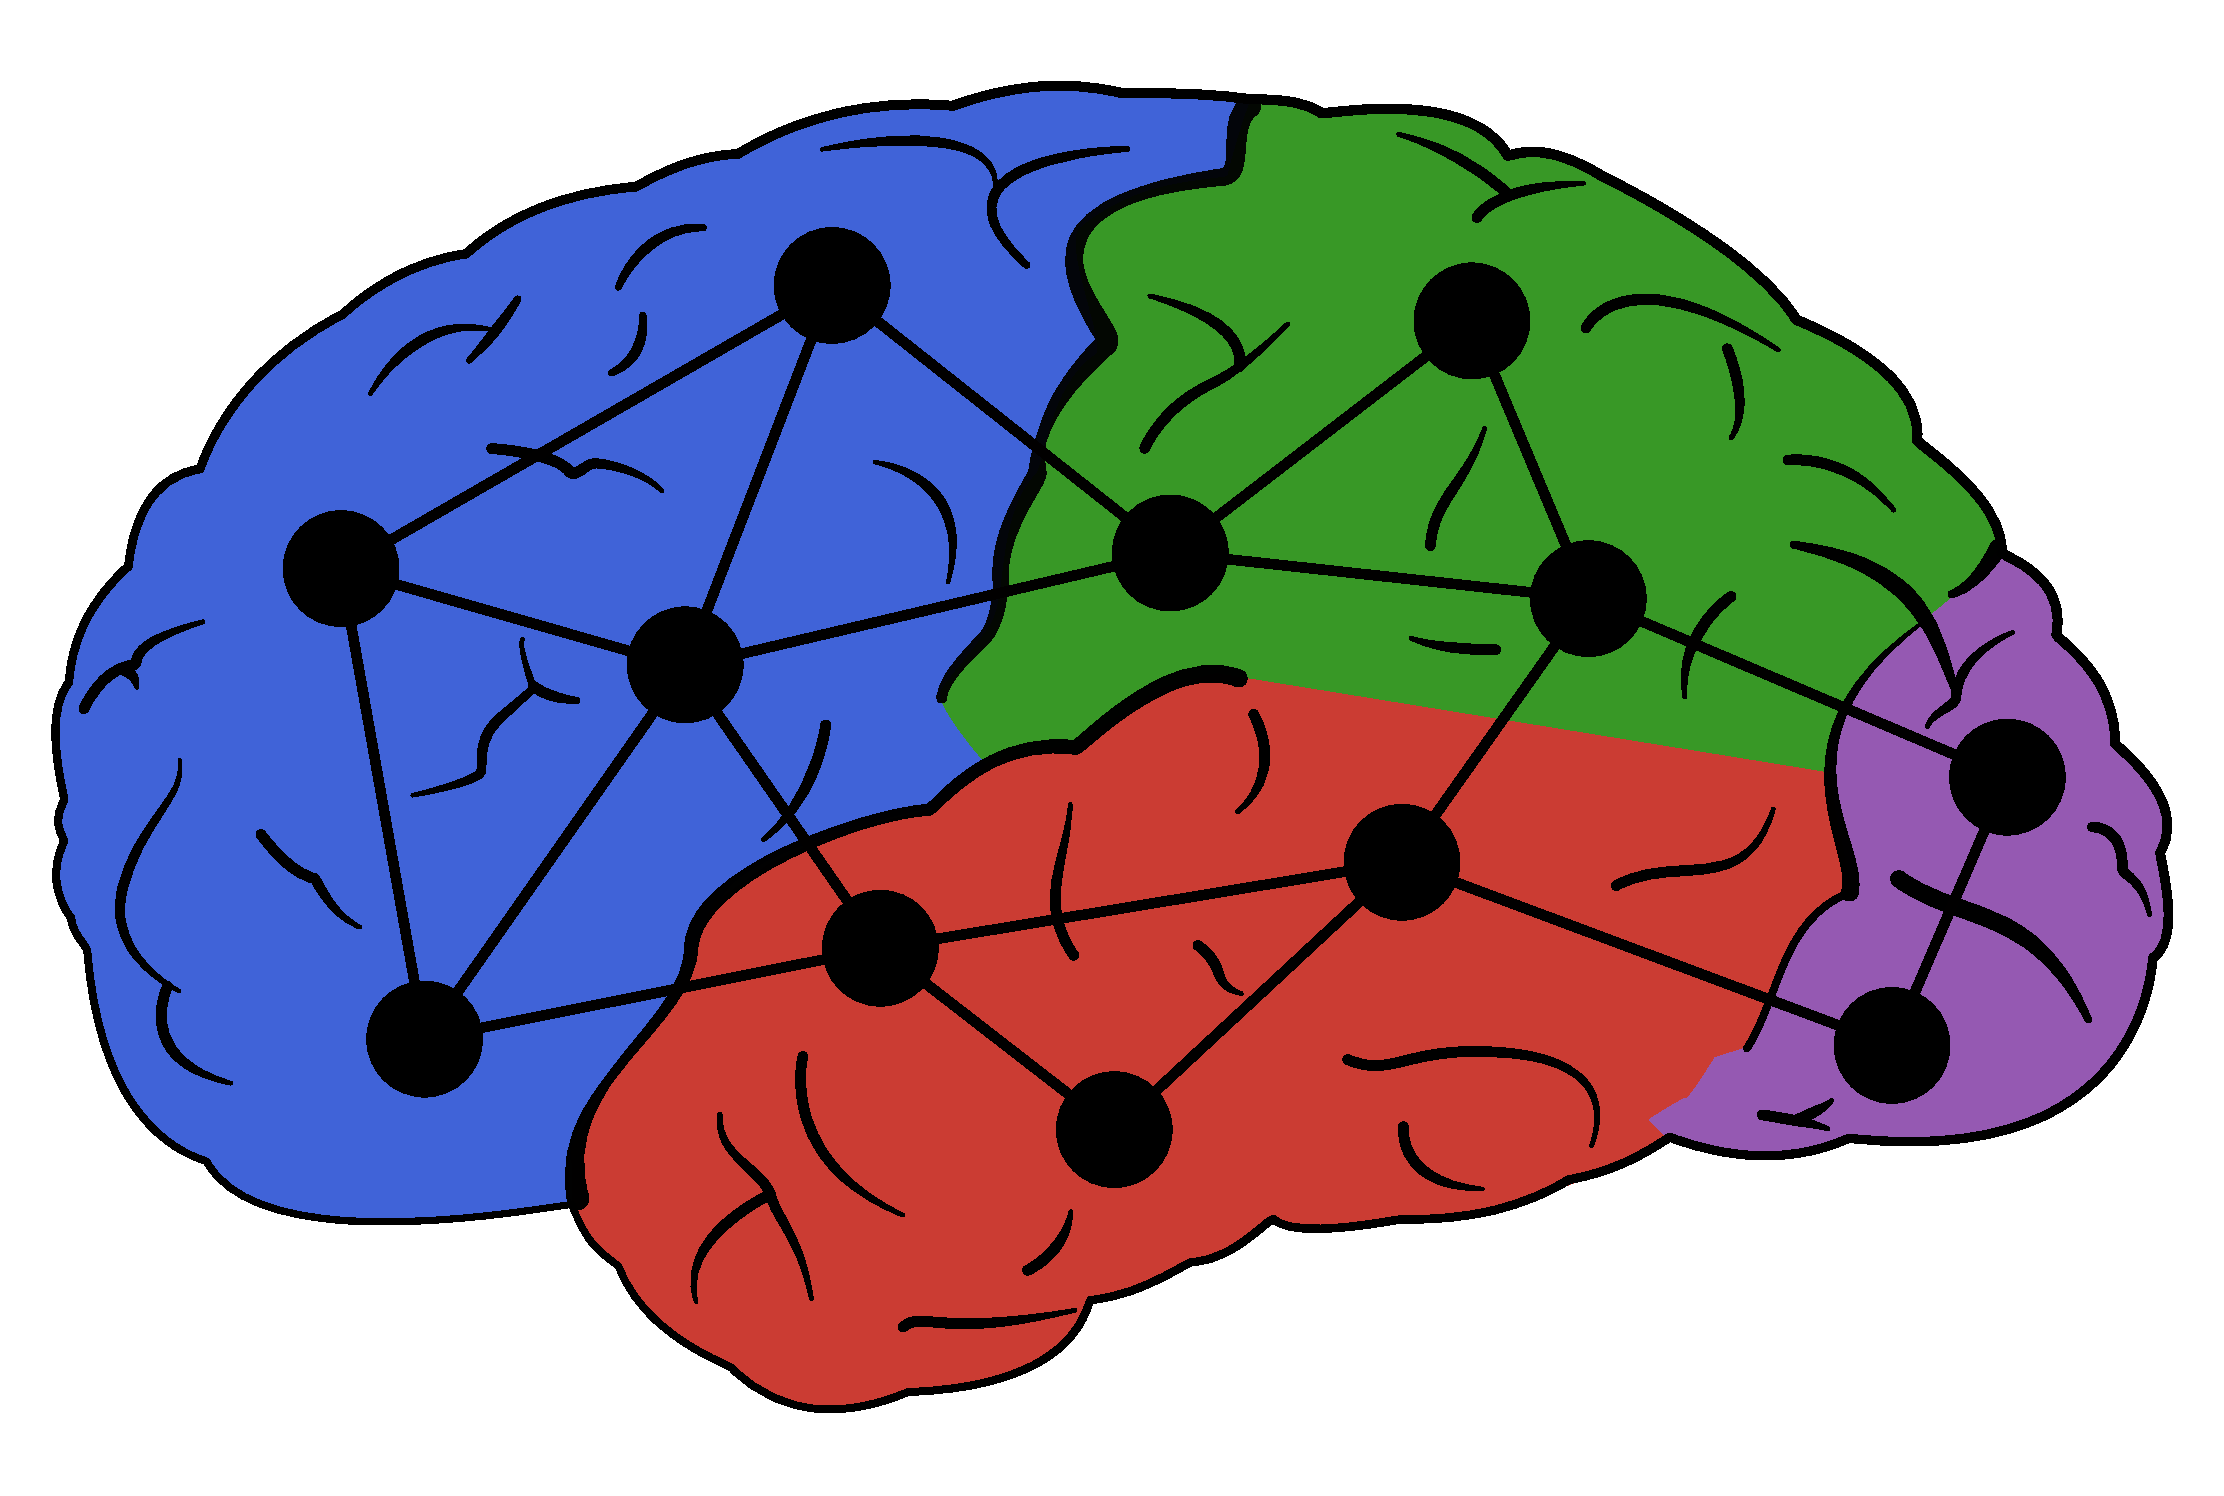
\includegraphics[width=5cm]{logo.pdf}}
    \caption{MINDFul.jl logo}
        \label{fig:logo}
    \end{figure}

\section{MINDFul.jl}
\verb|MINDFul.jl| is an open-source Julia library that provides a playground for \ac{MD} \ac{IBN}.
Although a minimal \ac{MD} \ac{IBN} framework is already implemented, users can extend the functionalities provided.
The library uses intent \acp{DAG} \cite{2023ChristouITG} to represent relationships between different intents.
This powerful scheme connects higher-level intents, which have a logical objective, with low-level intents, which are responsible for resource allocation, using a \ac{DAG}.
This hierarchical intent structure enables seamless interoperability between domains using \emph{intent delegation}, where an intent node is passed on to a different domain.

\verb|MINDFul.jl| is built with modularity in mind.
Intent state machines and algorithms can be alternated.
To evaluate different designs and algorithms under diverse scenarios, the appropriate interfaces are provided to facilitate simulations. 
The library offers a state representation of a common IP-optical network and an \ac{API} to access or modify it. 
The user can use these interfaces to conduct (event-based) simulations.
A company package, \verb|MINDFulMakie.jl|, can be used for some out-of-the-box visualizations like drawing an intent \ac{DAG} or visualizing a compiled connectivity intent in the network topology.
Finally, \verb|MINFulCompanion.jl| has been planned to contain a catalog of related algorithms and utilities.

The architecture provided by \verb|MINDFul.jl| is influenced by \cite{2013Rambach}.
The authors of this publication present a techno-economical overview of the equipment used in multilayer metro/core networks.
More specifically, we hold on to the pure IP-optical architecture signified by two layers; the electrical layer composed of IP routers and virtual links, and the optical layer composed of \acp{OXC} and physical fiber links.
Given the current technological advancements in coherent pluggable transceivers, like the OpenZR+ \ac{MSA} \cite{OpenZRProps}, we seek to also incorporate new trends into the represented architecture of the package.
A more detailed description of the modeling and architecture considered can be found in \cite{2022ChristouPlug}.

\section{Conclusion}
\verb|MINDFul.jl| is a Julia open-source library that facilitates research on \ac{MD} intent-driven IP-optical networks.
It provides a way to develop experimental intent system architectures and customized algorithms, as well as evaluate them using simulations and visualizations.
It fills a noticeable gap in the current openly-available tools.
We believe that the modular architecture, together with Julia's attributes, like speed and dynamicity, can significantly help advance the adaptation of \ac{IBN} in modern \ac{MD} networks.



%\begin{lstlisting}[language = Julia]
%using Plots
%
%x = -3.0:0.01:3.0
%y = rand(length(x))
%plot(x, y)
%\end{lstlisting}


%\begin{figure}[t]
%\centerline{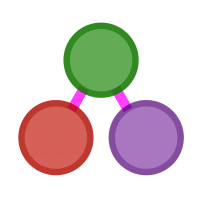
\includegraphics[width=4cm]{juliagraphs.png}}
%\caption{This is example of the image in a column.}
%	\label{fig:sample_figure}
%\end{figure}
%The figure \ref{fig:sample_figure} is taken from the JuliaGraphs
%organization \footnote{https://github.com/JuliaGraphs}.
%Just a citation \cite{bezanson2017julia}.

% **************GENERATED FILE, DO NOT EDIT**************

\bibliographystyle{juliacon}
\bibliography{ref.bib}


\end{document}

% Inspired by the International Journal of Computer Applications template
